\documentclass[a4paper]{book}\usepackage{graphicx, color}
%% maxwidth is the original width if it is less than linewidth
%% otherwise use linewidth (to make sure the graphics do not exceed the margin)
\makeatletter
\def\maxwidth{ %
  \ifdim\Gin@nat@width>\linewidth
    \linewidth
  \else
    \Gin@nat@width
  \fi
}
\makeatother

\definecolor{fgcolor}{rgb}{0.2, 0.2, 0.2}
\newcommand{\hlnumber}[1]{\textcolor[rgb]{0,0,0}{#1}}%
\newcommand{\hlfunctioncall}[1]{\textcolor[rgb]{0.501960784313725,0,0.329411764705882}{\textbf{#1}}}%
\newcommand{\hlstring}[1]{\textcolor[rgb]{0.6,0.6,1}{#1}}%
\newcommand{\hlkeyword}[1]{\textcolor[rgb]{0,0,0}{\textbf{#1}}}%
\newcommand{\hlargument}[1]{\textcolor[rgb]{0.690196078431373,0.250980392156863,0.0196078431372549}{#1}}%
\newcommand{\hlcomment}[1]{\textcolor[rgb]{0.180392156862745,0.6,0.341176470588235}{#1}}%
\newcommand{\hlroxygencomment}[1]{\textcolor[rgb]{0.43921568627451,0.47843137254902,0.701960784313725}{#1}}%
\newcommand{\hlformalargs}[1]{\textcolor[rgb]{0.690196078431373,0.250980392156863,0.0196078431372549}{#1}}%
\newcommand{\hleqformalargs}[1]{\textcolor[rgb]{0.690196078431373,0.250980392156863,0.0196078431372549}{#1}}%
\newcommand{\hlassignement}[1]{\textcolor[rgb]{0,0,0}{\textbf{#1}}}%
\newcommand{\hlpackage}[1]{\textcolor[rgb]{0.588235294117647,0.709803921568627,0.145098039215686}{#1}}%
\newcommand{\hlslot}[1]{\textit{#1}}%
\newcommand{\hlsymbol}[1]{\textcolor[rgb]{0,0,0}{#1}}%
\newcommand{\hlprompt}[1]{\textcolor[rgb]{0.2,0.2,0.2}{#1}}%

\usepackage{framed}
\makeatletter
\newenvironment{kframe}{%
 \def\at@end@of@kframe{}%
 \ifinner\ifhmode%
  \def\at@end@of@kframe{\end{minipage}}%
  \begin{minipage}{\columnwidth}%
 \fi\fi%
 \def\FrameCommand##1{\hskip\@totalleftmargin \hskip-\fboxsep
 \colorbox{shadecolor}{##1}\hskip-\fboxsep
     % There is no \\@totalrightmargin, so:
     \hskip-\linewidth \hskip-\@totalleftmargin \hskip\columnwidth}%
 \MakeFramed {\advance\hsize-\width
   \@totalleftmargin\z@ \linewidth\hsize
   \@setminipage}}%
 {\par\unskip\endMakeFramed%
 \at@end@of@kframe}
\makeatother

\definecolor{shadecolor}{rgb}{.97, .97, .97}
\definecolor{messagecolor}{rgb}{0, 0, 0}
\definecolor{warningcolor}{rgb}{1, 0, 1}
\definecolor{errorcolor}{rgb}{1, 0, 0}
\newenvironment{knitrout}{}{} % an empty environment to be redefined in TeX

\usepackage{alltt}
\usepackage{subfiles}
\usepackage{mathtools}
\usepackage{rotating}
\usepackage{graphicx}
\usepackage[authordate,backend=biber]{biblatex-chicago}
\usepackage[colorlinks=true,linkcolor=black,citecolor=black,urlcolor=black]{hyperref}

\title{Preliminary Thesis Defence\\~\\
\begin{tabular}{rl}
Supervisor:&Jean-Louis Arcand\footnote{Professor of Economics, The Graduate Institute, Geneva; Director, Centre for Finance and Development; jean-louis.arcand@graduateinstitute.ch}\\
Second Reader:&Lore Vandewalle\footnote{Assistant Professor of Economics, The Graduate Institute, Geneva; lore.vandewalle@graduateinstitute.ch}
\end{tabular}
}

\author{Bastiaan Quast\thanks{PhD Student, The Graduate Institute, Geneva; bastiaan.quast@graduateinstitute.ch / bquast@gmail.com}}

\let\oldmarginpar\marginpar
\renewcommand\marginpar[1]{\-\oldmarginpar[\raggedleft\footnotesize #1]
{\raggedright\footnotesize #1}}

\addglobalbib{bibliography.bib}

\newbibmacro{string+doiurlisbn}[1]{%
  \iffieldundef{doi}{%
    \iffieldundef{url}{%
      \iffieldundef{isbn}{%
        \iffieldundef{issn}{%
          #1%
        }{%
          \href{http://books.google.com/books?vid=ISSN\thefield{issn}}{#1}%
        }%
      }{%
        \href{http://books.google.com/books?vid=ISBN\thefield{isbn}}{#1}%
      }%
    }{%
      \href{\thefield{url}}{#1}%
    }%
  }{%
    \href{http://dx.doi.org/\thefield{doi}}{#1}%
  }%
}

\DeclareFieldFormat{title}{\usebibmacro{string+doiurlisbn}{\mkbibemph{#1}}}
\DeclareFieldFormat[article,incollection]{title}%
    {\usebibmacro{string+doiurlisbn}{\mkbibquote{#1}}}
\IfFileExists{upquote.sty}{\usepackage{upquote}}{} 


\begin{document}

\frontmatter
\maketitle
\tableofcontents

\chapter{Introduction}
jade

\mainmatter

\chapter{Additional South African Evidence on Pensions and Child Growth}

\section*{Abstract}

In this paper I look at the effect of the gender of pension recipients
on the growth of children in the same households.

I do this by comparing z-scores of anthropometrics of South African
children living in the same household as state pension recipients. This
paper exploits the fact that the data set consists of two surveys which
were done before and after the lowering of the pension eligibility age
for men to the same age as women.

The main preliminary finding is that the household effect was only
significant in 2012.

\section{Introduction}

This paper looks at the effect of the gender of pension recipients on
the growth of children in their household in South Africa. The approach
is very similar to Duflo
(\href{http://www.jstor.org/discover/10.2307/117257}{2000},\href{http://wber.oxfordjournals.org/content/17/1/1}{2003}).
The deviation from international standards
\href{http://www.who.int/childgrowth/en/}{Child Growth Standards} for
weight-for-height and length-for-age are computed as z-scores. These are
then compared for different pension recipient status.

The anthropometrics are useful for computing z-scores. These z-scores
are considered a good representation of short-term or long-term
malnutrition respectively, especially for children between 6 and 60
months old.

The South African pension is a useful variable to measure income because
of its criteria. Besides a maximum level of income, the only criterium
is the age of a person. Because of this the status as a recipient is
quite exogenous and there are few selection bias problems. The
problematic difference between the eligibility age of men and women was
eliminated between the two surveys which creates an interesting natural
experiment.

Duflo finds evidence in South Africa's 1993
\href{http://microdata.worldbank.org/index.php/catalog/297}{Integrated
Household Survey} that girls' short term nutrition (weight-for-height)
was positively influence by living with the maternal grandmother if the
grandmother was eligible for a state pension. This is directly after the
significant increase in the pension sum for blacks. The
pension-eligibility age at this time was 60 for women and 65 for men.

This study deviates from the Duflo study in several ways. In 2008 and
2012 the first and second wave of the
\href{http://www.nids.uct.ac.za/home/}{National Income Dynamics Study}
have gathered similar data. In the period 2008-2010, the government
lowered the eligibility age for men from 65 to 60
(\href{http://www.southafrica.info/services/government/pension-160708.htm}{Announcement}).

This happened in a few steps. As of July 16th 2008 men aged 63 and 64
were eligible for a pension. Men aged 61 and 62 became eligible in April
2009. Finally in January 2010, pension eligibility age was at 60 for all
citizens.

Another deviation is the usage of
\href{http://www.who.int/childgrowth/en/}{Child Growth Standards} in
stead of CDC's, since these have superseded the CDC charts, however this
should not be of any consequence.

The main preliminary result is that the household effect (i.e.~having
one or more recipients in the household) is very insignificant in the
2008 estimate. But in the 2012 estimate it is very significant.

\section{Data}

In this paper I use data from two sources. The first is the South
African National Income Dynamics Survey and the second is the World
Health Organization's Child Growth Standards
\href{http://www.who.int/childgrowth/en/}{Child Growth Standards}.

The main source of data is the NIDS. This survey collects data on a
representative set of appproximately 10,000 South African households.
The primary information types I use are, the child anthropometrics, the
age and gender of household members, and the status as state pension
recipients.

For adults several variables measure the different amounts and sources
of income. Among those, a variable if the adult receives a state
pension, and if so, how much. This is a numeric variable, the values of
which lie very close together. For simplicity I have temporarily used
this variable as a dummy.

Children's anthropometrics are taken, these are length/height, weight,
and waist. Using these anthropometics and WHO growth standards, z-scores
have been calculated. Unfortunately wave 2 (2012) accidentally omitted
the z-scores, so that these cannot be evaluated until an updated version
is published. However, I have computed the length-for-age z-scores
manually.

In 2006 the WHO published its standards for child growth
\href{http://www.who.int/childgrowth/en/}{Child Growth Standards}. These
standards are based on the scores of children from different ethnic
populations in households which observed a healthy lifestyle. The
standards provide the means and standards deviations used. These are on
a monthly basis for height-for-age, and on a semi-centimeter level for
weight-for-height scores.




\begin{knitrout}
\definecolor{shadecolor}{rgb}{0.969, 0.969, 0.969}\color{fgcolor}\begin{kframe}
\begin{alltt}
p1 <- \hlfunctioncall{ggplot}(\hlfunctioncall{subset}(w1_child, w1_woman_60 == 1), \hlfunctioncall{aes}(w1_c_age_m, w1_zhfa, colour = \hlfunctioncall{factor}(w1_c_woman)))
p1 + \hlfunctioncall{stat_smooth}(method = \hlstring{"loess"}) + \hlfunctioncall{geom_point}()
\end{alltt}


{\ttfamily\noindent\color{warningcolor}{\#\# Warning: Removed 324 rows containing missing values (stat\_smooth).}}

{\ttfamily\noindent\color{warningcolor}{\#\# Warning: Removed 263 rows containing missing values (stat\_smooth).}}

{\ttfamily\noindent\color{warningcolor}{\#\# Warning: Removed 51 rows containing missing values (stat\_smooth).}}

{\ttfamily\noindent\color{warningcolor}{\#\# Warning: Removed 638 rows containing missing values (geom\_point).}}\end{kframe}
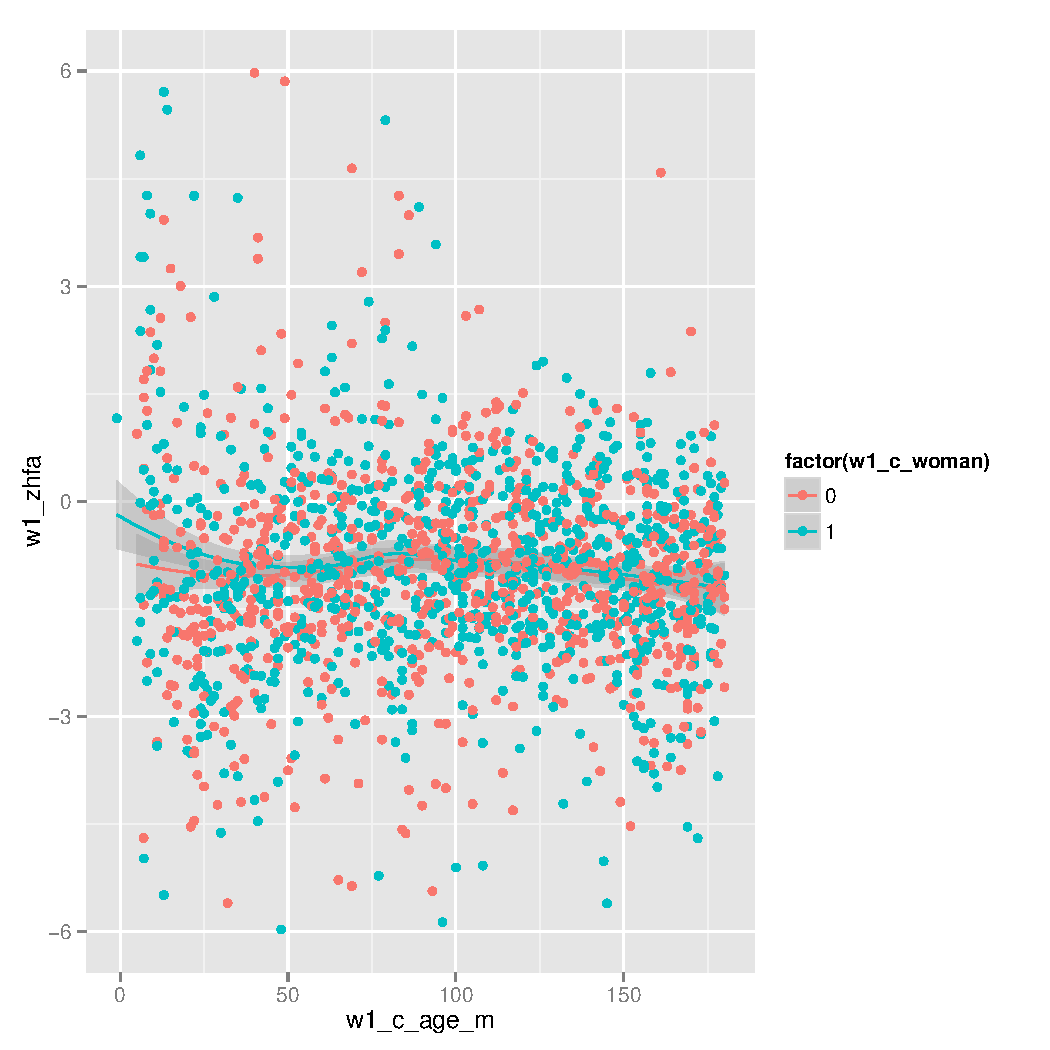
\includegraphics[width=\maxwidth]{figure/r-p1} 

\end{knitrout}


\section{Results}

Basic HAZ (2008)

\begin{knitrout}
\definecolor{shadecolor}{rgb}{0.969, 0.969, 0.969}\color{fgcolor}\begin{kframe}
\begin{alltt}
\hlfunctioncall{summary}(w1_haz0)
\end{alltt}
\begin{verbatim}
## 
## Call:
## lm(formula = w1_zhfa ~ w1_spen_w + w1_spen_m + w1_h_tinc + w1_best_edu + 
##     w1_best_age_yrs, data = w1_child, subset = w1_c_age_m >= 
##     6 & w1_c_age_m <= 60)
## 
## Residuals:
##    Min     1Q Median     3Q    Max 
## -4.779 -1.036 -0.169  0.834  7.060 
## 
## Coefficients:
##                  Estimate Std. Error t value Pr(>|t|)    
## (Intercept)     -1.43e+00   1.44e-01   -9.87   <2e-16 ***
## w1_spen_w        2.32e-02   1.15e-01    0.20   0.8402    
## w1_spen_m        1.36e-01   1.72e-01    0.79   0.4281    
## w1_h_tinc        3.62e-05   9.99e-06    3.62   0.0003 ***
## w1_best_edu      1.63e-03   7.84e-03    0.21   0.8355    
## w1_best_age_yrs  7.61e-03   3.64e-03    2.09   0.0369 *  
## ---
## Signif. codes:  0 '***' 0.001 '**' 0.01 '*' 0.05 '.' 0.1 ' ' 1
## 
## Residual standard error: 1.77 on 1436 degrees of freedom
##   (1936 observations deleted due to missingness)
## Multiple R-squared:  0.0134,	Adjusted R-squared:  0.00994 
## F-statistic: 3.89 on 5 and 1436 DF,  p-value: 0.00164
\end{verbatim}
\end{kframe}
\end{knitrout}


HAZ 2008, with 2012 eligiblity as an IV
\begin{knitrout}
\definecolor{shadecolor}{rgb}{0.969, 0.969, 0.969}\color{fgcolor}\begin{kframe}
\begin{alltt}
\hlfunctioncall{summary}(tsls_w1w2_haz0)
\end{alltt}
\begin{verbatim}
## 
##  2SLS Estimates
## 
## Model Formula: w1_zhfa ~ w1_spen_w + w1_spen_m + w1_h_tinc + w1_best_edu + w1_best_age_yrs
## 
## Instruments: ~w2_spen_w + w2_spen_m + w1_h_tinc + w1_best_edu + w1_best_age_yrs
## 
## Residuals:
##    Min. 1st Qu.  Median    Mean 3rd Qu.    Max. 
##  -4.990  -0.835  -0.050   0.000   0.788   7.070 
## 
##                   Estimate Std. Error t value Pr(>|t|)    
## (Intercept)     -1.172e+00  7.388e-02 -15.861  < 2e-16 ***
## w1_spen_w        1.748e-02  9.477e-02   0.184   0.8536    
## w1_spen_m       -1.374e-01  1.444e-01  -0.952   0.3414    
## w1_h_tinc        2.995e-05  5.606e-06   5.342 9.69e-08 ***
## w1_best_edu      2.410e-03  3.532e-03   0.682   0.4951    
## w1_best_age_yrs  4.127e-03  1.863e-03   2.215   0.0268 *  
## ---
## Signif. codes:  0 '***' 0.001 '**' 0.01 '*' 0.05 '.' 0.1 ' ' 1
## 
## Residual standard error: 1.4889 on 4227 degrees of freedom
\end{verbatim}
\end{kframe}
\end{knitrout}


HAZ 2008, with 2012 eligiblity as an IV (men over 65 only)
\begin{knitrout}
\definecolor{shadecolor}{rgb}{0.969, 0.969, 0.969}\color{fgcolor}\begin{kframe}
\begin{alltt}
\hlfunctioncall{summary}(tsls_w1w2_haz1)
\end{alltt}
\begin{verbatim}
## 
##  2SLS Estimates
## 
## Model Formula: w1_zhfa ~ w1_spen_w + w1_spen_m + w1_h_tinc + w1_best_edu + w1_best_age_yrs
## 
## Instruments: ~w2_spen_w + w2_spen_m_65 + w1_h_tinc + w1_best_edu + w1_best_age_yrs
## 
## Residuals:
##    Min. 1st Qu.  Median    Mean 3rd Qu.    Max. 
##  -4.990  -0.836  -0.050   0.000   0.786   7.040 
## 
##                   Estimate Std. Error t value Pr(>|t|)    
## (Intercept)     -1.173e+00  7.387e-02 -15.880  < 2e-16 ***
## w1_spen_w        8.576e-03  9.541e-02   0.090   0.9284    
## w1_spen_m       -9.189e-02  1.348e-01  -0.681   0.4956    
## w1_h_tinc        2.992e-05  5.605e-06   5.339 9.85e-08 ***
## w1_best_edu      2.443e-03  3.531e-03   0.692   0.4890    
## w1_best_age_yrs  4.092e-03  1.860e-03   2.200   0.0278 *  
## ---
## Signif. codes:  0 '***' 0.001 '**' 0.01 '*' 0.05 '.' 0.1 ' ' 1
## 
## Residual standard error: 1.4885 on 4227 degrees of freedom
\end{verbatim}
\end{kframe}
\end{knitrout}


\begin{refsection}
\chapter{Replication of: Surviving Andersonville}
\subfile{surviving.tex}
\printbibliography
\end{refsection}

\chapter{Single-Agent Belief Distributions}

\section*{Abstract}
By constructing a distribution of the belief structure of a single
agent, we can mitigate seemingly incommensurable beliefs. This paper
proposes to generalise the concept of a single agents beliefs, from a
point estimate to a distributional approximation. This will allow us to
deal with differing estimates of the probability \emph{p}, as well as
with estimates of \emph{p} and \emph{¬p} violating unitarity, in
meaningful way. Additionally with a distributional approximation, we can
estimate agents' beliefs, using the state which they are in.

\section{Introduction}

It generally held to be so that people sometimes hold beliefs which are
incommensurable with each other. In technical terms we could say, the
knowledge base is interally inconsistent. This incommensurability
becomes especially apparent when these beliefs are quantified.

As an example consider the following. If we have the probability of some
event \emph{e} occuring with probability \emph{p}. By definition, all
probabilities are exhausted at \emph{1}. Therefore the probability of
that event not occuring (i.e. \emph{¬p} or \emph{not p}) is \emph{1-p}.

\begin{quote}
¬p = 1 - p
\end{quote}

It is often observed, that people hold beliefs that do not meet this
condition, these beliefs can thus be described as:

\begin{quote}
¬p ≠ 1 - p
\end{quote}

In addition to this, we often see that people have different beliefs
about the same thing, often just moments apart (e.g.~beginning and end
of a survey). This could be the case for many (unrelated) reasons, such
as, fatigue, hunger, anchoring, etc. We can express this as:

\begin{quote}
p\_1(e) ≠ p\_2(e)
\end{quote}

We are thus faced with the fact that we get responses from agents

In this paper I describe how we can generalise the idea of perception of
probability -for a single agent- from a point estimate, to a
distributional approximation.

Doing this will allow us to deal with seemingly inconsistent beliefs in
a single framework in a \emph{meaningful} way.

\section{An example}

On a fair die, the chance of throwing 3 eyes is 16, call this \emph{p}.
The chance that you do not throw 3 eyes (i.e. \emph{¬p}) is therefore
\emph{1-p}, or

\begin{knitrout}
\definecolor{shadecolor}{rgb}{0.969, 0.969, 0.969}\color{fgcolor}\begin{kframe}
\begin{alltt}
1 - (1/6)
\end{alltt}
\begin{verbatim}
## [1] 0.8333
\end{verbatim}
\end{kframe}
\end{knitrout}


This is a very simple statistical exercise, and most people will be able
to give you the answer that I derived. The reason for this is that
people learn to use dice and how they operate, in e.g.~board games.
Likewise for coin flipping and many other basic statistical trials. In
this context, you would rarely find people accepting a bet that has a
negative expected value. Such as non-equal payout for a fair coin flip.

However, as soon as odds become less transparent, statistical methods
are often applied with less rigour. Especially when dealing with
observed implicit payout structures. As a results bets with negative
expected payouts, such as lotteries, are often accepted.

Let us continue with the idea of a lottery. For a lottery at the local
sports club, 100 tickets were printed, yet only 5 out of every 8 tickets
was sold, therefore tickets will be drawn until a winner is found. The
price of a ticket is 1 apple, and the prize for the winner is 50 apples.

Our victim is called Janus. After Janus buys a ticket for the lottery,
we ask him the following questions.

\begin{enumerate}
\def\labelenumi{\arabic{enumi}.}
\itemsep1pt\parskip0pt\parsep0pt
\item
  What is the chance (in percent) that you will win the lottery?
\item
  What is the chance (as a ratio) that someone else will win the
  lottery?
\item
  What is the chance that nobody wins the lottery?
\item
  You came with one apple, with how many apples do you expect to walked
  away?
\item
  What is the chance (as a ratio) that you will win the lottery?
\end{enumerate}

The first question is not very hard:

\begin{knitrout}
\definecolor{shadecolor}{rgb}{0.969, 0.969, 0.969}\color{fgcolor}\begin{kframe}
\begin{alltt}
1/(100 * (5 * 8))
\end{alltt}
\begin{verbatim}
## [1] 0.00025
\end{verbatim}
\end{kframe}
\end{knitrout}


But perhaps it is something you wouldn't always do without a calculator
or at least pen and paper. The second probability is:

Definitely something most people would do on paper. However, since we
are at the sports club, this is something we might not have at hand.

As can be seen, question (1) and (5) are identical. If you go through
the questions without having done the calculations beforehand, you will
likely be inclined to give a lower answer to (5) than you were to (1).
Presumable you would be quite neutral when answering question (1). Yet
the question preceding question (5) is rather negative, since you would
probably expect to walk away with zero apples, this would lead you to be
in a more negative mood when answering (5). Furthermore, you could have
become tired of answering so many questions, which generally diminishes
your perception of your chance of being successful.

Janus acts very much in accordance with our expectations, and gives us
the following responses.

\begin{enumerate}
\def\labelenumi{\arabic{enumi}.}
\itemsep1pt\parskip0pt\parsep0pt
\item
  2\% (has to be more than two)
\item
  19/20
\item
  0
\item
  0
\item
  1/60
\end{enumerate}

We observe two different estimates of the same \emph{p(e)}.

\begin{knitrout}
\definecolor{shadecolor}{rgb}{0.969, 0.969, 0.969}\color{fgcolor}\begin{kframe}
\begin{alltt}
p_1 = 1/100
p_1
\end{alltt}
\begin{verbatim}
## [1] 0.01
\end{verbatim}
\end{kframe}
\end{knitrout}


\begin{knitrout}
\definecolor{shadecolor}{rgb}{0.969, 0.969, 0.969}\color{fgcolor}\begin{kframe}
\begin{alltt}
p_2 = 1/60
p_2
\end{alltt}
\begin{verbatim}
## [1] 0.01667
\end{verbatim}
\end{kframe}
\end{knitrout}



Normally we would take either one of the responses, or such some other
way to come to a point estimate, such as averaging.

\section{As a distribution}

Let us assume that question (2) was answered in an slightly optimistic
state, and question 6 in a slightly pessimistic state. Furthermore, let
us assume that beliefs are normally distributed, and that these slightly
pessimistic and slightly optimistic state are each away from the mean,
below and above respectively. Lets express (5) as a number: 0.0167. We
can now construct the standard deviation.

\begin{knitrout}
\definecolor{shadecolor}{rgb}{0.969, 0.969, 0.969}\color{fgcolor}\begin{kframe}
\begin{alltt}
mu = p_1
mu
\end{alltt}
\begin{verbatim}
## [1] 0.01
\end{verbatim}
\end{kframe}
\end{knitrout}


\begin{knitrout}
\definecolor{shadecolor}{rgb}{0.969, 0.969, 0.969}\color{fgcolor}\begin{kframe}
\begin{alltt}
sigma = p_2 - mu
sigma
\end{alltt}
\begin{verbatim}
## [1] 0.006667
\end{verbatim}
\end{kframe}
\end{knitrout}


We can now define our subjects beliefs on winning the lottery as:

\begin{quote}
B\textasciitilde{}N(0.0167,0.00167)
\end{quote}

Let us now suppose that our subject loses his wallet before the winner
is drawn. If we want to predict how is beliefs have changed, we can for
example assume that they are now 2below is mean belief. This would thus
give us:

\begin{knitrout}
\definecolor{shadecolor}{rgb}{0.969, 0.969, 0.969}\color{fgcolor}\begin{kframe}
\begin{alltt}
mu - sigma
\end{alltt}
\begin{verbatim}
## [1] 0.003333
\end{verbatim}
\end{kframe}
\end{knitrout}


If however, Janus there after is in a euphoric state because he find his
wallet again, and on top of this a nice shiny green apple, than his new
belief might change to \emph{3s} above his mean level. Which would give
us:

\begin{knitrout}
\definecolor{shadecolor}{rgb}{0.969, 0.969, 0.969}\color{fgcolor}\begin{kframe}
\begin{alltt}
mu + 2 * sigma
\end{alltt}
\begin{verbatim}
## [1] 0.02333
\end{verbatim}
\end{kframe}
\end{knitrout}


\begin{quote}
p anp (1-p)
\end{quote}

How do we match the answers to questions (2) and (3), the chance that
Janus thinks he has of winning, with the chance that somebody else win
(i.e.~that he does not win). Let us write both odds as numbers:

\begin{quote}
p\_1 = 0.02 1 - p\_2 = 0.95 =\textgreater{} p\_2 = 0.05
\end{quote}

Let us suppose that the estimate of \emph{p} was positive by one and
that the estimate of \emph{1-p} was positive by \emph{3s} then we know:

% R Block

\section{An application}

Estimation of a 95\% confidence interval for a belief on probability,
how the lottery profit from this.

\section{Now\ldots{}for something much more important}

\href{http://www.youtube.com/watch?v=FVwtTrlPSSk}{A video of a penguin
being tickled}

\begin{refsection}
\chapter{Morris Shin Currency Attacks}
\subfile{morrisShin.tex}
\parencite{morris1998unique}
\printbibliography
\end{refsection}

\backmatter
\chapter{End notes}

\end{document}
